\vspace{12pt}
\section{Proton-dopant interaction}
The effect of dopant cations on proton mobility remains incompletely explained. Since the dopant's function is promoting proton incorporation into the lattice, then to a first approximation any trivalent dopant should work, given they do not affect the overall structure or stability of the lattice. Substitution of zirconium by a lower valency cation results in a local distortion of cubic symmetry due to both a difference of charge and a difference of ionic radius. In fact, Iwahara and associates suggested that, for barium cerate, dopants that distort the lattice the least would promote the highest proton conductivity \cite{IWAHARA1994}. In oxide ion conducting materials, conduction is generally improved when the dopant ionic radius is comparable to that of the ion it replaces \cite{Haile2003, Mogensen2004}. However, this has not necessarily been the case for other proton conductors, as the example of BaZrO$_3$ doped with yttrium ($r=90$ pm) shows much higher conductivity than when doped with either In ($r=80$pm) or Sc ($r=74.5$pm), which are much closer in radius to Zr ($r=72$ pm) \cite{Kreuer2004}. As a result, the vast majority of studies have focused on barium zirconate (BaZrO$_3$) doped with yttrium (Y) \cite{Fabbri2010a,Yamazaki2011,Tao2007,Sun2013,Hossain2017}. 

One possible explanation for this is that the ionic radius of the dopant cation in comparison to zirconium may contribute to the placement of larger dopant cations in the barium position. As shown in equation \ref{eq:back:bariumSubstitution}, this has been observed in barium cerate for dopant ionic radii larger than that of Nd$^{3+}$ \cite{Makovec1997}. Both atomistic simulations \cite{Davies1999, Wu2005} and experimental studies \cite{Wu2004} support the analysis that it is energetically favorable for dopants larger than Nd to substitute for barium. 

Since this structural argument seems incomplete in explaining the higher conductivity in the case of yttrium-doped barium zirconate, it would seem the local chemical environment of the dopant may itself have an effect. In particular, association between the proton and the dopant ion has a much more important influence than simply ionic radius mismatch and lattice distortion itself. Proton trapping is the tendency for protons that are at oxygen sites adjacent to dopant ions to have decreased mobility due to the lower potential energy from the dopant's lower oxidation state \cite{Islam2004}. Atomistic simulations by Stokes and Islam \cite{Stokes2010} found that the proton would swing towards the dopant ion as shown in Figure \ref{fig:back:protonTrapping}, but that the extent of this pivot was different for each dopant, with gadolinium producing the smallest distortion of this proton from a neutral position in the lattice. Going further, the authors calculated a binding energy of a proton-dopant pair from examining the energy difference when these two types of defects were isolated in the lattice and when they were together in the same unit cell. The distance between proton and dopant correlated with the calculations of binding energy suggesting this possible route to explain the proton dopant sites.  
\begin{figure}
    \centering
    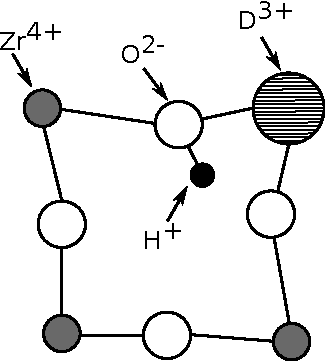
\includegraphics{Figures/BaZrO_3-dopant-lattice-strain.pdf}
    \caption{Model view of the lattice strain and positioning of a proton defect in an ``trap'' site near a dopant ion.}
    \label{fig:back:protonTrapping}
\end{figure}

The suitability of gadolinium as a dopant in barium zirconate was tested early on by Ryu and Haile \cite{Ryu1999} due to its success in providing high proton conductivity to barium cerate. The hope was that by adding barium zirconate to barium cerate the chemical stability could be improved. Gadolinium is also a successful dopant in ceria \cite{Infortuna2008, Steele2001}, albeit one that promotes oxide ion conduction rather than proton conduction in that case. But the low conductivity results of these early studies in comparison to yttrium doping resulted in much focus being devoted to yttrium. Kreuer's comparisons of Y- and Gd-doped barium zirconate showed an order of magnitude lower conductivity for Gd doping \cite{Kreuer2001}. Competing studies within a year of each other by Giannici put gadolinium in the list of ``good'' dopants in contrast to indium and scandium \cite{Giannici2010} while Imishuku showed gadolinium along with In and Sc with an order of magnitude lower conductivity than yttrium which was the highest of the series of dopants tested \cite{Imashuku2009}. 

Running in parallel to these studies were promising results for yttrium doped barium zirconate. Indeed, the highest proton conductivity of any species yet reported in the intermediate temperature range is Y-doped barium zirconate thin films produced by pulsed laser deposition. These epitaxially grown thin films demonstrated that the poor conductivity initially reported for barium zirconate owed to its small sized grains when produced as bulk pellets with the typical solid state reaction or sol-gel methods \cite{Pergolesi2010}. But in addition to the atomistic simulations by Stokes and Islam discussed above \cite{Stokes2010}, experimental evidence of proton trapping in yttrium-doped barium zirconate was demonstrated by Yamazaki in 2013 \cite{Yamazaki2013}. Both of these investigations explicitly suggested further investigation into Gd and Yb, as they may lead to reduced proton trapping at the dopant site, possibly resulting in as much as a factor of 2 improvement in conductivity in the case of gadolinium. Following this debate, Traversa's group tested a wide range of dopants, and Gd again emerged as a good candidate for dopants in bulk preparations due to not only good bulk conductivity but also denser grain growth in comparison to other dopants. It was again noted that gadolinium doped barium zirconate needs further investigation \cite{Gilardi2017}. It is in this context that we proceed with our investigation to contribute to this field.